\begin{enumerate}[label=\thesection.\arabic*.,ref=\thesection.\theenumi]
\numberwithin{equation}{enumi}

\item
Nichols chart is the plot of gain and phase that is the magnitude(in dB) on the vertical axis and phase(in deg) on the horizontal axis for the given transfer function. It is called the gain phase plot. These plots are used for the stability analysis of the system.
\\
There are four cases for finding the stability (r is magnitude in dB and $\phi$ is phase in deg)
\\
Case 1 : System with no unstable pole.
\\
For the stable function T(s) whose Nichols plot intersects dB line at least one time.The system is stable if and only if one of the following holds
\\
1) the steady gain $\mid ko\mid$ is less than 0 dB
\\
2) The Nichols plot T(j$\omega$) intersects the line segment C := [($\phi$,r) : r = 0 dB , $-180\degree$ \textless $\phi$ \textless $180\degree$ ]for the function with the positive steady gain ko and $\mid ko\mid$ larger than dB.
\\
Case 2: System with one unstable pole.
\\
The system is stable if and only if the half part of the Nichols plot crosses the line segment  C := [($\phi$,r) : r = 0 dB , $-180\degree$ \textless $\phi$ \textless $180\degree$], the steady gain ko is negative and $\mid ko\mid$ is larger than 0 dB.
\\
Case 3 : System with 2k unstable poles.
\\
The feedback system is stable if and only if the plot intersects the line segment C := [($\phi$,r) : r = 0 dB , $-180\degree$ \textless $\phi$ \textless $180\degree$], the steady gain ko is positive and $\mid ko\mid$  is larger than
0 dB
\\
Case 4 : System with 2k+1 unstable poles.
\\
The stability analysis of the system with 2k+1 unstable poles is equivalent to
that of the shifting Nichols plot of the function with one unstable pole.
\\
Consider the closed loop transfer function
\begin{align}
T(s) &= \frac{G(s)}{1+G(s)H(s)}
\label{eq:es17btech11009_CLTF}
\end{align}
The system flow is shown below

\begin{figure}[!ht]
	\begin{center}
		\resizebox{\columnwidth}{!}{\input{./figs/es17btech11009_1.tex}}
	\end{center}
\caption{}
\label{fig:es17btech11009_flow}
\end{figure}
Also, for the percentage overshoot(PO) we need the characteristic equation of the function so as to determine the damping ratio.
The general characteristic equations is 
\begin{align}
 s^2 + 2\zeta \omega  s + \omega ^2 
\label{es17btech11009_char}
\end{align}
where $\zeta$ is the damping ratio and $\omega$ is the natural frequency.
\\
Since all the systems above are third order or fourth order systems we need to decompose them into first order and second order to find out the PO.
\begin{align}
PO = \exp{\frac{-\zeta \pi}{\sqrt{1- \zeta^2}}} * 100
\label{es17btech11009_po}
\end{align}

\subsection{Stability}
\item
Using Nichol's chart , find out whether each of the system below are stable or not 
\begin{align}
G_{1}(s)= \frac{50}{s(s+3)(s+6)}
\label{eq:es17btech11009_a}
\\
 H_{1}(s)= 1
 \label{eq:es17btech11009_b}
\end{align}
\begin{align}
G_{2}(s)= \frac{9}{s^2(s+3)}
\label{eq:es17btech11009_c}
\\
 H_{2}(s)= (s+4)
 \label{eq:es17btech11009_d}
\end{align}
\begin{align}
G_{3}(s)= \frac{20}{s(s+1)}
\label{eq:es17btech11009_e}
\\
 H_{3}(s)= \frac{s+3}{s+4}
 \label{eq:es17btech11009_f}
\end{align}
\begin{align}
G_{4}(s)= \frac{100(s+5)}{s(s^2+4)(s+3)}
\label{eq:es17btech11009_g}
\\
 H_{4}(s)= 1
 \label{eq:es17btech11009_h}
\end{align}

For the above systems also estimate the percentage overshoot that can be expected when a step input is given to the system.
\item
From \eqref{eq:es17btech11009_a} and \eqref{eq:es17btech11009_b},
\begin{align}
G_{1}\brak{s}H_{1}\brak{s}&= \frac{50}{s\brak{s+3}\brak{s+6}}
\label{eq:es17btech11009_aa}
\end{align}
\solution
 From \eqref{eq:es17btech11009_CLTF},
 \begin{align}
T_{1}\brak{s} = \frac{50}{s^3 + 9s^2 + 18s + 50}
\label{eq:es17btech11009_11}
 \end{align}
\begin{lstlisting}
codes/es17btech11009_1.py
\end{lstlisting}
The above code gives the following plot for the closed loop system as shown in Fig \ref{fig:es17btech11009_fig1}
\begin{figure}[!h]
\centering
\includegraphics[width=\columnwidth]{./figs/es17btech11009_1.eps}
\caption{}
\label{fig:es17btech11009_fig1}
\end{figure}
The given system has no unstable poles so according to case 1, we could conclude that the plot satisfies the stability condition therefore, the system is stable.

\item
From \eqref{eq:es17btech11009_11},
There are no zeroes and poles are shown in Table \ref{table:es17btech11009_t1}

\begin{table}[!ht]
\centering
\input{./tables/es17btech11009_t1.tex}
\caption{}
\label{table:es17btech11009_t1}
\end{table}
Since we have two conjugate poles, The approximated transfer function is
\begin{align}
T\brak{s} = \frac{K_1}{\brak{s-p_{2}}\brak{s-p_{3}}}
\end{align}
\begin{align}
    T\brak{s}= \frac{K_{1}}{s^2 + 1.5s + 6.66}
    \label{eq:es17btech11009_aptf1}
\end{align}
The characteristic equation of \eqref{eq:es17btech11009_aptf1} is,
\begin{align}
 s^2 + 1.5s + 6.66 = 0
 \end{align}
From \eqref{es17btech11009_char} and \eqref{es17btech11009_po},
\\
 $\zeta$ = 0.29 and $\omega$ = 2.58
 \\
 Percentage overshoot = 38.4\%
 \item
The following code generates step response of the function \eqref{eq:es17btech11009_11} as shown in Fig \ref{fig:es17btech11009_fig11}
\begin{lstlisting}
codes/es17btech11009_11.py
\end{lstlisting}
\begin{figure}[!h]
\centering
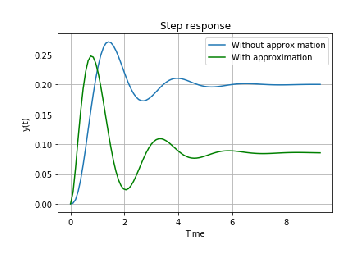
\includegraphics[width=\columnwidth]{./figs/es17btech11009_11.eps}
\caption{}
\label{fig:es17btech11009_fig11}
\end{figure}

\item
From \eqref{eq:es17btech11009_c} and \eqref{eq:es17btech11009_d},
\begin{align}
G_{2}\brak{s}H_{2}\brak{s}&= \frac{9\brak{s+4}}{s^2\brak{s+3}}
\label{eq:es17btech11009_bb}
\end{align}
\solution
 From \eqref{eq:es17btech11009_CLTF},
 \begin{align}
T_{2}\brak{s} = \frac{9}{s^3 + 3s^2 + 9s + 36}
\label{eq:es17btech11009_21}
 \end{align}
\begin{lstlisting}
codes/es17btech11009_2.py
\end{lstlisting}
The above code gives the following plot for the closed loop system as shown in Fig \ref{fig:es17btech11009_fig2}
\begin{figure}[!h]
\centering
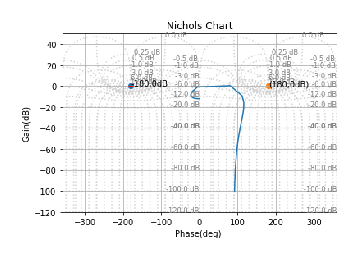
\includegraphics[width=\columnwidth]{./figs/es17btech11009_2.eps}
\caption{}
\label{fig:es17btech11009_fig2}
\end{figure}
The given system has two unstable poles so according to case 3, we could conclude that the system in unstable.
\item
From \eqref{eq:es17btech11009_21},
there are no zeroes and poles are shown in Table \ref{table:es17btech11009_t2}

\begin{table}[!ht]
\centering
\input{./tables/es17btech11009_t2.tex}
\caption{}
\label{table:es17btech11009_t2}
\end{table}
Since we have two conjugate poles, The approximated transfer function is
\begin{align}
T\brak{s} = \frac{K_1}{\brak{s-p_{2}}\brak{s-p_{3}}}
\end{align}
\begin{align}
    T\brak{s}= \frac{K_1}{s^2 + 0.42s + 10.28}
    \label{eq:es17btech11009_aptf2}
\end{align}
The characteristic equation of \eqref{eq:es17btech11009_aptf2} is,
\begin{align}
s^2 + 0.42s + 10.28 = 0
 \end{align}
From \eqref{es17btech11009_char} and \eqref{es17btech11009_po},
\\
 $\zeta$ = 0.065 and $\omega$ = 3.2
 \\
 Percentage overshoot = 81.8\%
 \item
The following code generates step response of the function \eqref{eq:es17btech11009_21} as shown in Fig \ref{fig:es17btech11009_fig21}
\begin{lstlisting}
codes/es17btech11009_21.py
\end{lstlisting}
\begin{figure}[!h]
\centering
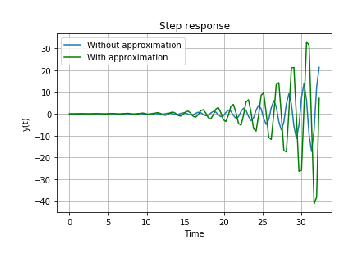
\includegraphics[width=\columnwidth]{./figs/es17btech11009_21.eps}
\caption{}
\label{fig:es17btech11009_fig21}
\end{figure}

\item
From \eqref{eq:es17btech11009_e} and \eqref{eq:es17btech11009_f},
\begin{align}
G_{3}\brak{s}H_{3}\brak{s}&= \frac{20\brak{s+3}}{s\brak{s+1}\brak{s+4}}
\label{eq:es17btech11009_cc}
\end{align}
\solution
From \eqref{eq:es17btech11009_CLTF},
 \begin{align}
T_{3}\brak{s} = \frac{20\brak{s+4}}{s^3 + 5s^2 + 24s + 60}
\label{eq:es17btech11009_31}
 \end{align}

\begin{lstlisting}
codes/es17btech11009_3.py
\end{lstlisting}
The above code gives the following plot of the closed loop system as shown in Fig \ref{fig:es17btech11009_fig3}
\begin{figure}[!h]
\centering
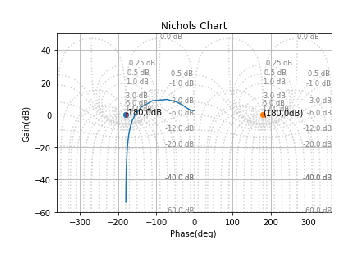
\includegraphics[width=\columnwidth]{./figs/es17btech11009_3.eps}
\caption{}
\label{fig:es17btech11009_fig3}
\end{figure}
The given system has no unstable poles so according to case 1, we could conclude that the plot satisfies the stability condition.The system is stable. 
\item
From \eqref{eq:es17btech11009_31},
The zeros and the poles are shown in Table \ref{table:es17btech11009_t3} 

\begin{table}[!ht]
\centering
\input{./tables/es17btech11009_t3.tex}
\caption{}
\label{table:es17btech11009_t3}
\end{table}
Since we have two conjugate poles, The approximated transfer function is
\begin{align}
T\brak{s} = \frac{K_1}{\brak{s-p_2}\brak{s-p_3}}
\end{align}
\begin{align}
    T\brak{s}= \frac{K_1}{s^2 + 1.72s + 18.28}
    \label{eq:es17btech11009_aptf3}
\end{align}
The characteristic equation of \eqref{eq:es17btech11009_aptf3} is,
\begin{align}
s^2 + 1.72s + 18.28 = 0
 \end{align}
From \eqref{es17btech11009_char} and \eqref{es17btech11009_po},
\\
 $\zeta$ = 0.201 and $\omega$ = 4.27
 \\
 Percentage overshoot = 52.2\%
 \item
The following code generates step response of the function \eqref{eq:es17btech11009_31} as shown in Fig \ref{fig:es17btech11009_fig31}
\begin{lstlisting}
codes/es17btech11009_31.py
\end{lstlisting}
\begin{figure}[!h]
\centering
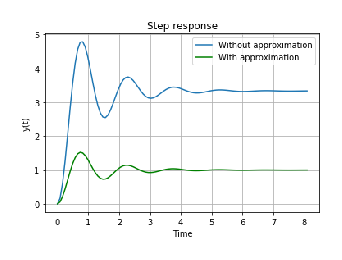
\includegraphics[width=\columnwidth]{./figs/es17btech11009_31.eps}
\caption{}
\label{fig:es17btech11009_fig31}
\end{figure}
\item
From \eqref{eq:es17btech11009_g} and \eqref{eq:es17btech11009_h},
\begin{align}
G_{4}\brak{s}H_{4}\brak{s}&= \frac{100\brak{s+5}}{s\brak{s^2+4}\brak{s+3}}
\label{eq:es17btech11009_dd}
\end{align}
\solution
From \eqref{eq:es17btech11009_CLTF},
\begin{align}
T_{4}\brak{s} = \frac{100\brak{s+5}}{s^4 + 3s^3 + 4s^2 + 112s + 500}
\label{eq:es17btech11009_41}
 \end{align}
\begin{lstlisting}
codes/es17btech11009_4.py
\end{lstlisting}
The above code gives the following plot for the closed loop system as shown in Fig \ref{fig:es17btech11009_fig4}.
\begin{figure}[!h]
\centering
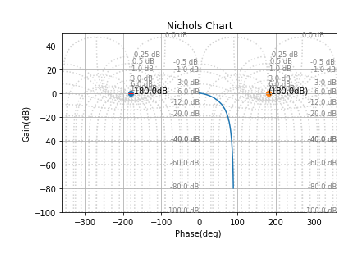
\includegraphics[width=\columnwidth]{./figs/es17btech11009_4.eps}
\caption{}
\label{fig:es17btech11009_fig4}
\end{figure}
The given system has 2 unstable poles so according to case 3, we could conclude that the system is unstable.
\item
From \eqref{eq:es17btech11009_41},
The zeroes and poles are shown in Table \ref{table:es17btech11009_t4}

\begin{table}[!ht]
\centering
\input{./tables/es17btech11009_t4.tex}
\caption{}
\label{table:es17btech11009_t4}
\end{table}
We have four conjugate poles, Consider the approximated transfer function 
\begin{align}
T\brak{s} = \frac{K_1}{\brak{s-p_{3}}\brak{s-p_{4}}}
\end{align}
\begin{align}
    T\brak{s}= \frac{K_1}{s^2 + 5.08s + 25.89}
    \label{eq:es17btech11009_aptf4}
\end{align}
The characteristic equation of \eqref{eq:es17btech11009_aptf4} is,
\begin{align}
s^2 + 1.72s + 18.28 = 0
 \end{align}
From \eqref{es17btech11009_char} and \eqref{es17btech11009_po},
\\
 $\zeta$ = 0.5 and $\omega$ = 5.08
 \\
 Percentage overshoot = 16.36\%

 \item
The following code generates step response of the function \eqref{eq:es17btech11009_41} as shown in Fig \ref{fig:es17btech11009_fig41}
\begin{lstlisting}
codes/es17btech11009_41.py
\end{lstlisting}
\begin{figure}[!h]
\centering
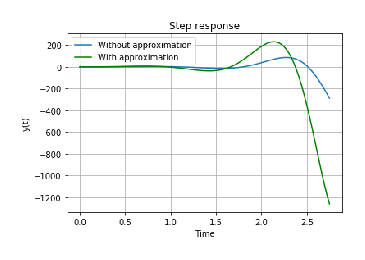
\includegraphics[width=\columnwidth]{./figs/es17btech11009_41.eps}
\caption{}
\label{fig:es17btech11009_fig41}
\end{figure}

\subsection{Range of K}
\item
Using Nichol's chart, find out the range of K for which the closed loop systems will be stable
\begin{align}
G_{5}(s)= \frac{K}{s(s+6)}
\label{eq:es17btech11009_i}
\\
 H_{5}(s)= \frac{1}{s+9}
 \label{eq:es17btech11009_j}
\end{align}
\begin{align}
G_{6}(s)= \frac{K(s+2)(s+4)}{s^2 - 3s +10}
\label{eq:es17btech11009_k}
\\
 H_{6}(s)= \frac{1}{s}
 \label{eq:es17btech11009_l}
\end{align}
\begin{align}
G_{7}(s)= \frac{K}{(s+1)(s+3)}
\label{eq:es17btech11009_m}
\\
 H_{7}(s)= \frac{s+5}{s+7}
 \label{eq:es17btech11009_n}
\end{align}
For the above systems also estimate the percentage overshoot that can be expected when a step input is given to the system.
\item
From \eqref{eq:es17btech11009_i} and \eqref{eq:es17btech11009_j},
\begin{align}
G_{5}\brak{s}H_{5}\brak{s}&= \frac{K}{s\brak{s+6}\brak{s+9}}
\label{eq:es17btech11009_ee}
\end{align}
\solution
From \eqref{eq:es17btech11009_CLTF},
\begin{align}
T_{5}\brak{s} = \frac{K\brak{s+9}}{s^3 +15s^2 +54s + K}
\label{eq:es17btech11009_51}
 \end{align}

\begin{lstlisting}
codes/es17btech11009_5.py
\end{lstlisting}

The above code gives the following plot for k = 2  as shown in Fig \ref{fig:es17btech11009_fig5}
\begin{figure}[!h]
\centering
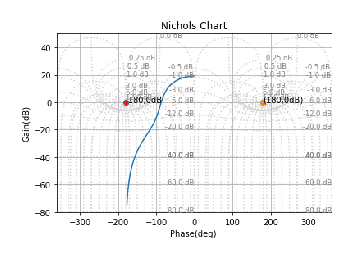
\includegraphics[width=\columnwidth]{./figs/es17btech11009_5.eps}
\caption{}
\label{fig:es17btech11009_fig5}
\end{figure}

By increasing k, we could see that the plot shifts in upward direction, so the range of k for which the system is stable is 0 \textless K \textless 810.
\item
Let k= 500

From \eqref{eq:es17btech11009_41},
The zeroes and poles are shown in Table \ref{table:es17btech11009_t5}

\begin{table}[!ht]
\centering
\input{./tables/es17btech11009_t5.tex}
\caption{}
\label{table:es17btech11009_t5}
\end{table}
Since we have two conjugate poles, Consider the approximated transfer function 
\begin{align}
T\brak{s} = \frac{K_1}{\brak{s-p_{2}}\brak{s-p_{3}}}
\end{align}

\begin{align}
    T\brak{s}= \frac{K_1}{s^2 + 1.26s + 36.39}
    \label{eq:es17btech11009_aptf5}
\end{align}
The characteristic equation of \eqref{eq:es17btech11009_aptf5} is,
\begin{align}
s^2 + 1.26s + 36.39 =0
 \end{align}
From \eqref{es17btech11009_char} and \eqref{es17btech11009_po},
\\
 $\zeta$ = 0.1 and $\omega$ =6.03 
 \\
 Percentage overshoot = 72.9\%

 \item
The following code generates step response of the function \eqref{eq:es17btech11009_51} as shown in Fig \ref{fig:es17btech11009_fig51}
\begin{lstlisting}
codes/es17btech11009_51.py
\end{lstlisting}
\begin{figure}[!h]
\centering
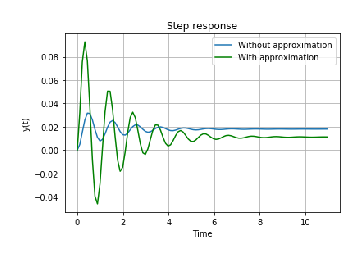
\includegraphics[width=\columnwidth]{./figs/es17btech11009_51.eps}
\caption{}
\label{fig:es17btech11009_fig51}
\end{figure}

\item
From \eqref{eq:es17btech11009_k} and \eqref{eq:es17btech11009_l},
\begin{align}
G_{6}\brak{s}H_{6}\brak{s}&= \frac{K\brak{s+2}\brak{s+4}}{s\brak{s^2 - 3s +10}}
\label{eq:es17btech11009_ff}
\end{align}
\solution
From \eqref{eq:es17btech11009_CLTF}
\begin{align}
T_{6}\brak{s} = \frac{K\brak{s^3 + 6s^2+8s}}{\brak{s^3 - 3s^2 + 10s }+\brak{s^2 +6s +8} K}
\label{eq:es17btech11009_61}
 \end{align}

\begin{lstlisting}
codes/es17btech11009_6.py
\end{lstlisting}
The above code gives the following plot for k = 5 as shown in Fig \ref{fig:es17btech11009_fig6}
\begin{figure}[!h]
\centering
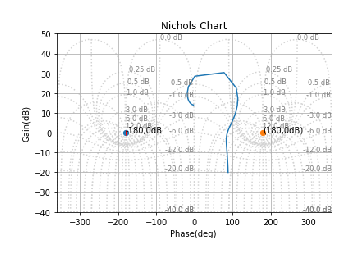
\includegraphics[width=\columnwidth]{./figs/es17btech11009_6.eps}
\caption{}
\label{fig:es17btech11009_fig6}
\end{figure}

By increasing k, we could see that the plot shifts in upward direction, so the range of k for which the system is stable is 3.9 \textless K \textless $\infty$.
\item
Let k= 5

From \eqref{eq:es17btech11009_61},
The zeros and poles are shown in Table \ref{table:es17btech11009_t6}

\begin{table}[!ht]
\centering
\input{./tables/es17btech11009_t6.tex}
\caption{}
\label{table:es17btech11009_t6}
\end{table}
Since we have two conjugate poles, Consider the approximated transfer function 
\begin{align}
T\brak{s} = \frac{K_1}{\brak{s-p_{2}}\brak{s-p_{3}}}
\end{align}

\begin{align}
    T\brak{s}= \frac{K_1}{s^2 + 0.96s + 38.9}
    \label{eq:es17btech11009_aptf6}
\end{align}
The characteristic equation of \eqref{eq:es17btech11009_aptf6} is,
\begin{align}
s^2 + 0.96s + 38.9=0
 \end{align}
From \eqref{es17btech11009_char} and \eqref{es17btech11009_po},
\\
 $\zeta$ =0.07 and $\omega$ = 6.23
 \\
 Percentage overshoot = 81\%

 \item
The following code generates step response of the function \eqref{eq:es17btech11009_61} as shown in Fig \ref{fig:es17btech11009_fig61}
\begin{lstlisting}
codes/es17btech11009_61.py
\end{lstlisting}
\begin{figure}[!h]
\centering
\includegraphics[width=\columnwidth]{./figs/es17btech11009_61.eps}
\caption{}
\label{fig:es17btech11009_fig61}
\end{figure}

\item
From \eqref{eq:es17btech11009_m} and \eqref{eq:es17btech11009_n},
\begin{align}
G_{7}\brak{s}H_{7}\brak{s}&= \frac{K}{\brak{s+1}\brak{s+3}\brak{s+5}\brak{s+7}}
\label{eq:es17btech11009_gg}
\end{align}
\solution
From \eqref{eq:es17btech11009_CLTF},
\begin{align}
T_{7}\brak{s} = \frac{K\brak{s^2 + 12s +35}}{\brak{s^4 + 16s^3 + 86s^2 + 176s + 105+K}}
\label{eq:es17btech11009_71}
 \end{align}

\begin{lstlisting}
codes/es17btech11009_7.py
\end{lstlisting}

The above code gives the following plot for k = 10 as shown in Fig \ref{fig:es17btech11009_fig7}

\begin{figure}[!h]
\centering
\includegraphics[width=\columnwidth]{./figs/es17btech11009_7.eps}
\caption{}
\label{fig:es17btech11009_fig7}
\end{figure}

By varying k, we could see that the  the range of k for which the system is stable is 3 \textless K \textless $\infty$.
\item
Let k= 1000

From \eqref{eq:es17btech11009_71},
The zeros and poles are shown in Table \ref{table:es17btech11009_t7}

\begin{table}[!ht]
\centering
\input{./tables/es17btech11009_t7.tex}
\caption{}
\label{table:es17btech11009_t7}
\end{table}
Since we have four conjugate poles, Consider the approximated transfer function 
\begin{align}
T\brak{s} = \frac{K_1}{\brak{s-p_{3}}\brak{s-p_{4}}}
\end{align}

\begin{align}
    T\brak{s}= \frac{K_1}{s^2 + 0.56s + 13.39}
    \label{eq:es17btech11009_aptf7}
\end{align}
The characteristic equation of \eqref{eq:es17btech11009_aptf7} is,
\begin{align}
s^2 + 0.56s + 13.39=0
 \end{align}
From \eqref{es17btech11009_char} and \eqref{es17btech11009_po},
\\
 $\zeta$ =0.076 and $\omega$ = 3.65
 \\
 Percentage overshoot = 79.4\%

 \item
The following code generates step response of the function \eqref{eq:es17btech11009_71} as shown in Fig \ref{fig:es17btech11009_fig71}
\begin{lstlisting}
codes/es17btech11009_71.py
\end{lstlisting}
\begin{figure}[!h]
\centering
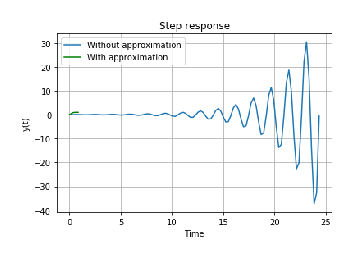
\includegraphics[width=\columnwidth]{./figs/es17btech11009_71.eps}
\caption{}
\label{fig:es17btech11009_fig71}
\end{figure}
  
\subsection{Closed Loop Frequency Response }
\item
For unity feedback (negative) systems given below, obtain closed loop frequency response using constant M and N circles.
\begin{align}
G_8(s)= \frac{10}{s(s+1)(s+2)}
 \label{eq:es17btech11009_o}
 \\
G_9(s)= \frac{1000}{(s+3)(s+4)(s+5)(s+6)}
\label{eq:es17btech11009_p}
\\
G_0(s)= \frac{50(s+3)}{s(s+2)(s+4)}
\label{eq:es17btech11009_q}
\end{align}
For the above systems also estimate the percentage overshoot that can be expected when a step input is given to the system.

\textbf{Constant M and N Circles}
\\
Let $G(j\omega)$ be complex quantity it can be written as 
\begin{align}
G\brak{j \omega} &= x+j y
\label{eq:es17btech11009_comp}
\end{align}
where x,y are real quantities.

M circles are called constant magnitude Loci and N circles are called as
constant phase angle Loci.These are helpful in determining the closed-loop frequency response of unity negative feedback systems. \\
\textbf{Mcircle(Constant-Magnitude Loci):} 

Let M be magnitude of closed loop transfer function. From \eqref{eq:es17btech11009_comp}
\begin{align}
M &= \abs{\frac{x+j Y}{1+x+j y}}
\\
M^{2} &= \frac{x^{2}+y^{2}}{\brak{1+x}^{2}+y^{2}}
\label{eq:es17btech11009_constm}
\end{align}

Hence,
\begin{align}
X^{2}\brak{1-M^{2}}-2M^{2}X-M^{2}+\brak{1-M^{2}}Y^{2} &= 0
\label{eq:es17btech11009_cm1}
\end{align}

If $M=1$, then from Equation \eqref{eq:es17btech11009_constm}, we obtain $x =\frac{-1}{2}$ This is the equation of a straight line parallel to the Y axis and passing through the point $\brak{\frac{-1}{2},0}$.

If $M \neq 1$ Equation \eqref{eq:es17btech11009_cm1} can be written as
\begin{align}
x^{2}+\frac{2M^{2}}{M^{2}-1}x+\frac{M^{2}}{M^{2}-1}+y^{2} &= 0
\end{align}

Simplifying,
\begin{align}
\brak{x+\frac{M^{2}}{M^{2}-1}}^{2}+y^{2} &= \frac{M^{2}}{\brak{M^{2}-1}^{2}}
\label{eq:es17btech11009_cm2}
\end{align}

Equation \eqref{eq:es17btech11009_cm2} is the equation of a circle with center 
$\brak{-\frac{M^{2}}{M^{2}-1},0}$ and radius $\abs{\frac{M}{M^{2}-1}}$

Thus the intersection of Nquist plot with M circle at a frequency($\omega$) results as the magnitude of closed loop transfer function as M at frequency ($\omega$)
\textbf{N Circles(Constant-Phase-Angle Loci):}
Finding Phase angle $\alpha$ from \eqref{eq:es17btech11009_constm} we get,
\begin{align}
\alpha &= \tan^{-1}\brak{\frac{y}{x}}-\tan^{-1}\brak{\frac{y}{1+x}}
\\
\text{Let } tan\alpha &= N
\\
N &= tan\brak{\tan^{-1}\brak{\frac{y}{x}}-\tan^{-1}\brak{\frac{y}{1+x}}}
\end{align}
Simplifying,
\begin{align}
N &= \frac{y}{x^{2}+x+y^{2}}
\end{align}
Further Simplifying..
\begin{align}
\brak{x+\frac{1}{2}}^{2}+\brak{y-\frac{1}{2N}}^{2} &= \frac{1}{4}+\frac{1}{\brak{2N}^{2}}
\label{eq:es17btech11009_cm4}
\end{align}
Equation \eqref{eq:es17btech11009_cm4} is the equation of a circle with center at $\brak{\frac{-1}{2},\frac{1}{2N}}$ and radius $\sqrt{\frac{1}{4}+\frac{1}{\brak{2N}^{2}}}$
Thus the intersection of Nquist plot with N circle at a frequency($\omega$) results as the phase of closed loop transfer function as $tan^{-1}\brak{N}$ at frequency ($\omega$)
\item
From \eqref{eq:es17btech11009_o},
\begin{align}
G_{8}\brak{s} &=\frac{10}{s\brak{s+1}\brak{s+2}}
\label{eq:es17btech1109_hh}
\end{align}
\solution 
From \eqref{eq:es17btech11009_CLTF},
\begin{align}
T_{8}\brak{s} &=\frac{10}{s^3 + 3s^2 + 2s +10}
\label{eq:es17btech11009_81}
\end{align}
The following code gives the nichol plot of \eqref{eq:es17btech11009_81} shown in Fig \ref{fig:es17btech11009_fig8}
\begin{lstlisting}
codes/es17btech11009_8.py
\end{lstlisting}
\begin{figure}[!h]
\includegraphics[width=\columnwidth]{./figs/es17btech11009_8.eps}
\caption{}
\label{fig:es17btech11009_fig8}
\end{figure}
The M and N circles of T($j\omega$) in the gain phase plane are transformed into M and N contours in rectangular co-ordinates. A point on the constant M loci in T($j\omega$) plane is transferred to gain phase plane by drawing the vector directed from the origin of T($j\omega$) plane to a particular point on M circle and then measuring the length in dB and angle in degree.
\item
The following code plots  M and N contours in rectangle co-ordinates look like as shown in Fig. \ref{fig:es17btech11009_8_1}.
\begin{lstlisting}
codes/es17btech11009_8_code1.py
\end{lstlisting}

\begin{figure}[!h]
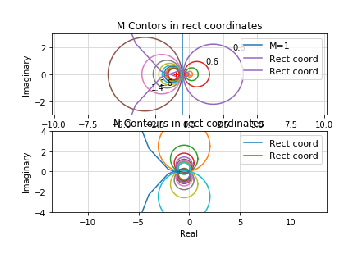
\includegraphics[width=\columnwidth]{./figs/es17btech11009_8_fig1.eps}
\caption{}
\label{fig:es17btech11009_8_1}
\end{figure}
\item
To find the intersection of M and N contours in the rectangle co-ordinates at different frequencies. \\
\solution 
The following code finds intersection of M and N contours with rectangular co-ordinates at different frequencies
\begin{lstlisting}
codes/es17btech11009_8_code2.py
\end{lstlisting}
The points M and frequencies are listed in Table  \ref{table:es17btech11009_table1}
\begin{table}[!ht]
\centering
\input{./tables/es17btech11009_table1.tex}
\caption{}
\label{table:es17btech11009_table1}
\end{table}
\item
The points N and frequencies are listed in Table\ref{table:es17btech11009_table2}
\begin{table}[!ht]
\centering
\input{./tables/es17btech11009_table2.tex}
\caption{}
\label{table:es17btech11009_table2}
\end{table}
The constant N locus for given value of $\alpha$ is not the entire circle but only an arc.This is beacuse tangent of angle remains same if $+180\degree$ or 
$-180\degree$ is added to the angle.
\item
From \eqref{eq:es17btech11009_81},

The zeroes and poles are shown in Table \ref{table:es17btech11009_t8}

\begin{table}[!ht]
\centering
\input{./tables/es17btech11009_t8.tex}
\caption{}
\label{table:es17btech11009_t8}
\end{table}
Since we have two conjugate poles, Consider the approximated transfer function 
\begin{align}
T\brak{s} = \frac{K_1}{\brak{s-p_{1}}\brak{s-p_{2}}}
\end{align}

\begin{align}
    T\brak{s}= \frac{K_1}{s^2 + 0.3s + 3}
    \label{eq:es17btech11009_aptf8}
\end{align}
The characteristic equation of \eqref{eq:es17btech11009_aptf8} is,
\begin{align}
s^2 + 0.3s + 3=0
 \end{align}
From \eqref{es17btech11009_char} and \eqref{es17btech11009_po},
\\
 $\zeta$ =0.0086 and $\omega$ = 1.732
 \\
 Percentage overshoot = 75.5\%

 \item
The following code generates step response of the function \eqref{eq:es17btech11009_81} as shown in Fig \ref{fig:es17btech11009_fig81}
\begin{lstlisting}
codes/es17btech11009_81.py
\end{lstlisting}
\begin{figure}[!h]
\centering
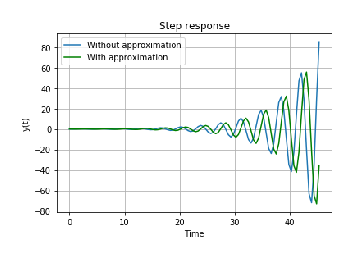
\includegraphics[width=\columnwidth]{./figs/es17btech11009_81.eps}
\caption{}
\label{fig:es17btech11009_fig81}
\end{figure}
  
\item
From \eqref{eq:es17btech11009_p},
\begin{align}
G_{9}\brak{s} &=\frac{1000}{\brak{s+3}\brak{s+4}\brak{s+5}\brak{s+6}}
\label{eq:es17btech11009_ii}
\end{align}
\solution
From \eqref{eq:es17btech11009_CLTF}, 
\begin{align}
T_9\brak{s} &=\frac{1000}{s^4 + 18s^3 + 119s^2 + 342s + 1360}
\label{eq:es17btech11009_91}
\end{align}
The following code gives the nichols plot as shown in Fig \ref{fig:es17btech11009_fig9}
\begin{lstlisting}
codes/es17btech11009_9.py
\end{lstlisting}
\begin{figure}[!h]
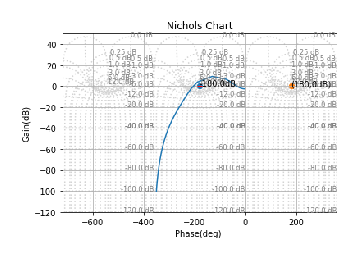
\includegraphics[width=\columnwidth]{./figs/es17btech11009_9.eps}
\caption{}
\label{fig:es17btech11009_fig9}
\end{figure}
\item
The following code plots  M and N contours in rectangle co-ordinates which look like as shown in Fig. \ref{fig:es17btech11009_9_1}.

\begin{lstlisting}
codes/es17btech11009_9_code1.py
\end{lstlisting}
\begin{figure}[!h]
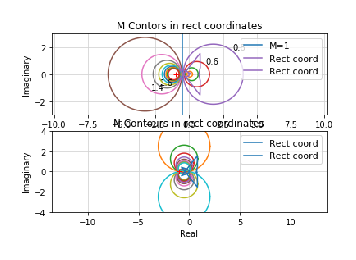
\includegraphics[width=\columnwidth]{./figs/es17btech11009_9_fig1.eps}
\caption{}
\label{fig:es17btech11009_9_1}
\end{figure}
\item 
The following code finds intersection of M and N contours with rectangular co-ordinates at different frequencies
\begin{lstlisting}
codes/es17btech11009_9_code2.py
\end{lstlisting}
The points M and frequencies are listed in Table  \ref{table:es17btech11009_table3}
\begin{table}[!ht]
\centering
\input{./tables/es17btech11009_table3.tex}
\caption{}
\label{table:es17btech11009_table3}
\end{table}
\item
The points N and frequencies are listed in Table\ref{table:es17btech11009_table4}
\begin{table}[!ht]
\centering
\input{./tables/es17btech11009_table4.tex}
\caption{}
\label{table:es17btech11009_table4}
\end{table}
\item
From \eqref{eq:es17btech11009_71},

The zeroes and poles are shown in Table \ref{table:es17btech11009_t9}

\begin{table}[!ht]
\centering
\input{./tables/es17btech11009_t9.tex}
\caption{}
\label{table:es17btech11009_t9}
\end{table}
We have four conjugate poles, Consider the approximated transfer function 
\begin{align}
T\brak{s} = \frac{K_1}{\brak{s-p_{3}}\brak{s-p_{4}}}
\end{align}

\begin{align}
    T\brak{s}= \frac{K_1}{s^2 + 0.56s + 13.39}
    \label{eq:es17btech11009_aptf9}
\end{align}
The characteristic equation of \eqref{eq:es17btech11009_aptf9} is,
\begin{align}
s^2 + 0.56s + 13.39=0
 \end{align}
From \eqref{es17btech11009_char} and \eqref{es17btech11009_po},
\\
 $\zeta$ =0.11 and $\omega$ = 3.91
 \\
 Percentage overshoot = 71\%

 \item
The following code generates step response of the function \eqref{eq:es17btech11009_91} as shown in Fig \ref{fig:es17btech11009_fig91}
\begin{lstlisting}
codes/es17btech11009_91.py
\end{lstlisting}
\begin{figure}[!h]
\centering
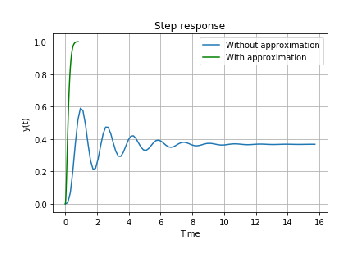
\includegraphics[width=\columnwidth]{./figs/es17btech11009_91.eps}
\caption{}
\label{fig:es17btech11009_fig91}
\end{figure}
\item
From \eqref{eq:es17btech11009_q},
\begin{align}
G_0\brak{s} &=\frac{50\brak{s+3}}{s\brak{s+2}\brak{s+4}}
\label{eq:es17btech11009_jj}
\end{align}
\solution
From \eqref{eq:es17btech11009_CLTF},
\begin{align}
T_0\brak{s} &=\frac{50\brak{s+3}}{s^3 + 6s^2 + 58s +150}
\label{eq:es17btech11009_101}
\end{align}
 
The following code gives the nichols plot as shown in Fig \ref{fig:es17btech11009_fig10}
\begin{lstlisting}
codes/es17btech11009_10.py
\end{lstlisting}
\begin{figure}[!h]
\includegraphics[width=\columnwidth]{./figs/es17btech11009_10.eps}
\caption{}
\label{fig:es17btech11009_fig10}
\end{figure}
\item
The following code plots  M and N contours in rectangle co-ordinates which look like as shown in Fig. \ref{fig:es17btech11009_10_1}.
\begin{lstlisting}
codes/es17btech11009_10_code1.py
\end{lstlisting}
\begin{figure}[!h]
\includegraphics[width=\columnwidth]{./figs/es17btech11009_10_fig1.eps}
\caption{}
\label{fig:es17btech11009_10_1}
\end{figure}
\item
The following code finds intersection of M and N contours with rectangular co-ordinates at different frequencies
\begin{lstlisting}
codes/es17btech11009_10_code2.py
\end{lstlisting}
The points M and frequencies are listed in Table  \ref{table:es17btech11009_table5}
\begin{table}[!ht]
\centering
\input{./tables/es17btech11009_table5.tex}
\caption{}
\label{table:es17btech11009_table5}
\end{table}
\item
The points N and frequencies are listed in Table\ref{table:es17btech11009_table6}
\begin{table}[!ht]
\centering
\input{./tables/es17btech11009_table6.tex}
\caption{}
\label{table:es17btech11009_table6}
\end{table}
\item
From \eqref{eq:es17btech11009_101},
The zeroes and poles are shown in Table \ref{table:es17btech11009_t10}

\begin{table}[!ht]
\centering
\input{./tables/es17btech11009_t10.tex}
\caption{}
\label{table:es17btech11009_t10}
\end{table}
Since we have two conjugate poles, Consider the approximated transfer function 
\begin{align}
T\brak{s} = \frac{K_1}{\brak{s-p_{2}}\brak{s-p_{3}}}
\end{align}

\begin{align}
    T\brak{s}= \frac{K_1}{s^2 + 2.92s + 48.91}
    \label{eq:es17btech11009_aptf10}
\end{align}
The characteristic equation of \eqref{eq:es17btech11009_aptf10} is,
\begin{align}
s^2 + 2.92s + 48.91=0
 \end{align}
From \eqref{es17btech11009_char} and \eqref{es17btech11009_po},
\\
 $\zeta$ =0.2 and $\omega$ = 6.99
 \\
 Percentage overshoot = 52.7\%

 \item
The following code generates step response of the function \eqref{eq:es17btech11009_101} as shown in Fig \ref{fig:es17btech11009_fig101}
\begin{lstlisting}
codes/es17btech11009_101.py
\end{lstlisting}
\begin{figure}[!h]
\centering
\includegraphics[width=\columnwidth]{./figs/es17btech11009_101.eps}
\caption{}
\label{fig:es17btech11009_fig101}
\end{figure}
  
\end{enumerate}